\begin{anexosenv}

\partanexos

% Texto do primeiro anexo.

\chapter{\nmu Figuras}
\label{anexos}

% \begin{figure}[h]
%   \centering
% 	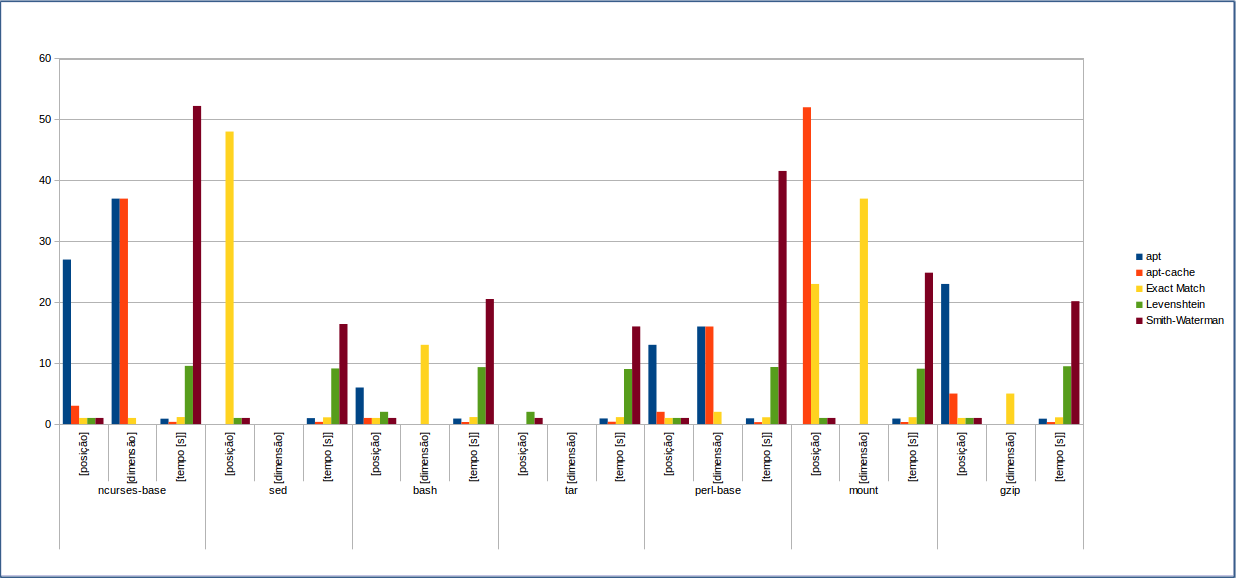
\includegraphics[width=0.7\textheight,angle=90]{figuras/grafico}
%   \caption{Amostra de comparação dos resultados}
%   \label{fig:figuras_grafico}
% \end{figure}
% \cleardoublepage

% \begin{figure}[h]
%   \centering
% 	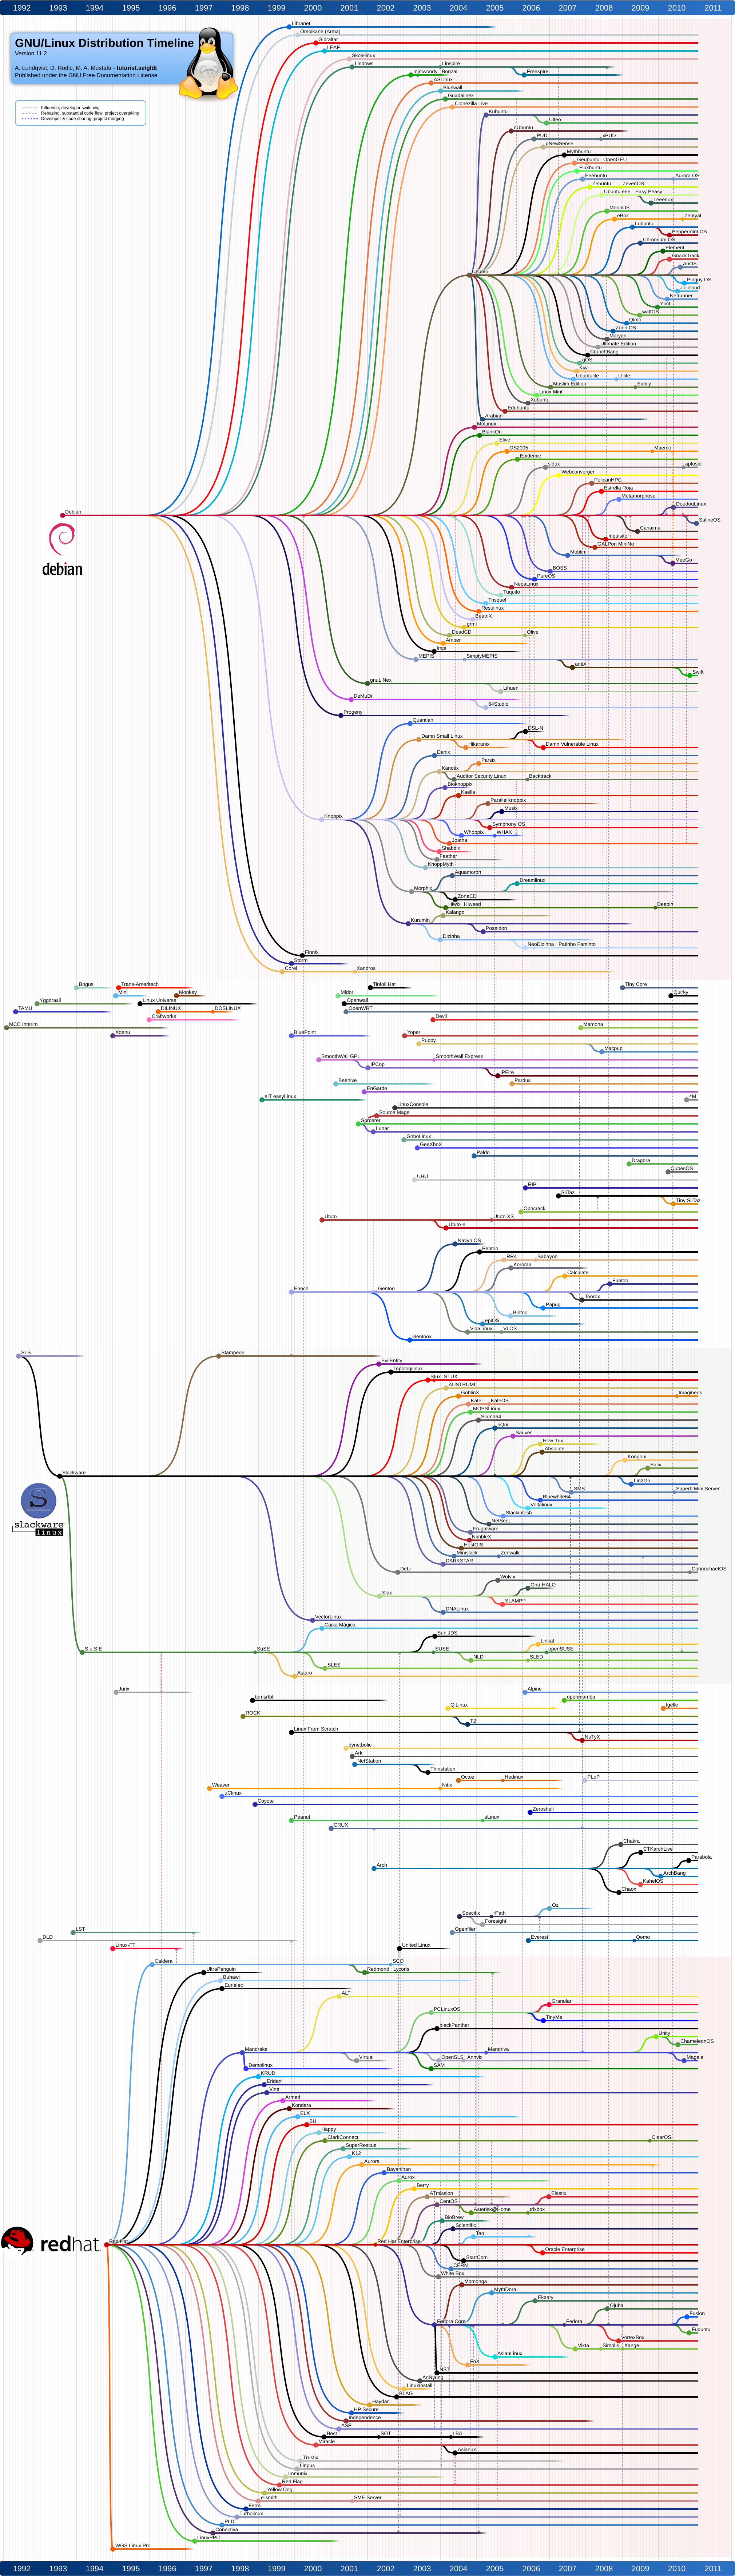
\includegraphics[width=0.75\textwidth]{figuras/linux-timeline-heranca}
%   \caption[Heranças de algumas das distribuições Linux existentes hoje]{Heranças de algumas das distribuições Linux existentes hoje\protect\footnotemark.}
%   \label{fig:figuras_linux_timeline_heranca}
% \end{figure}

\begin{figure}[h]
  \centering
	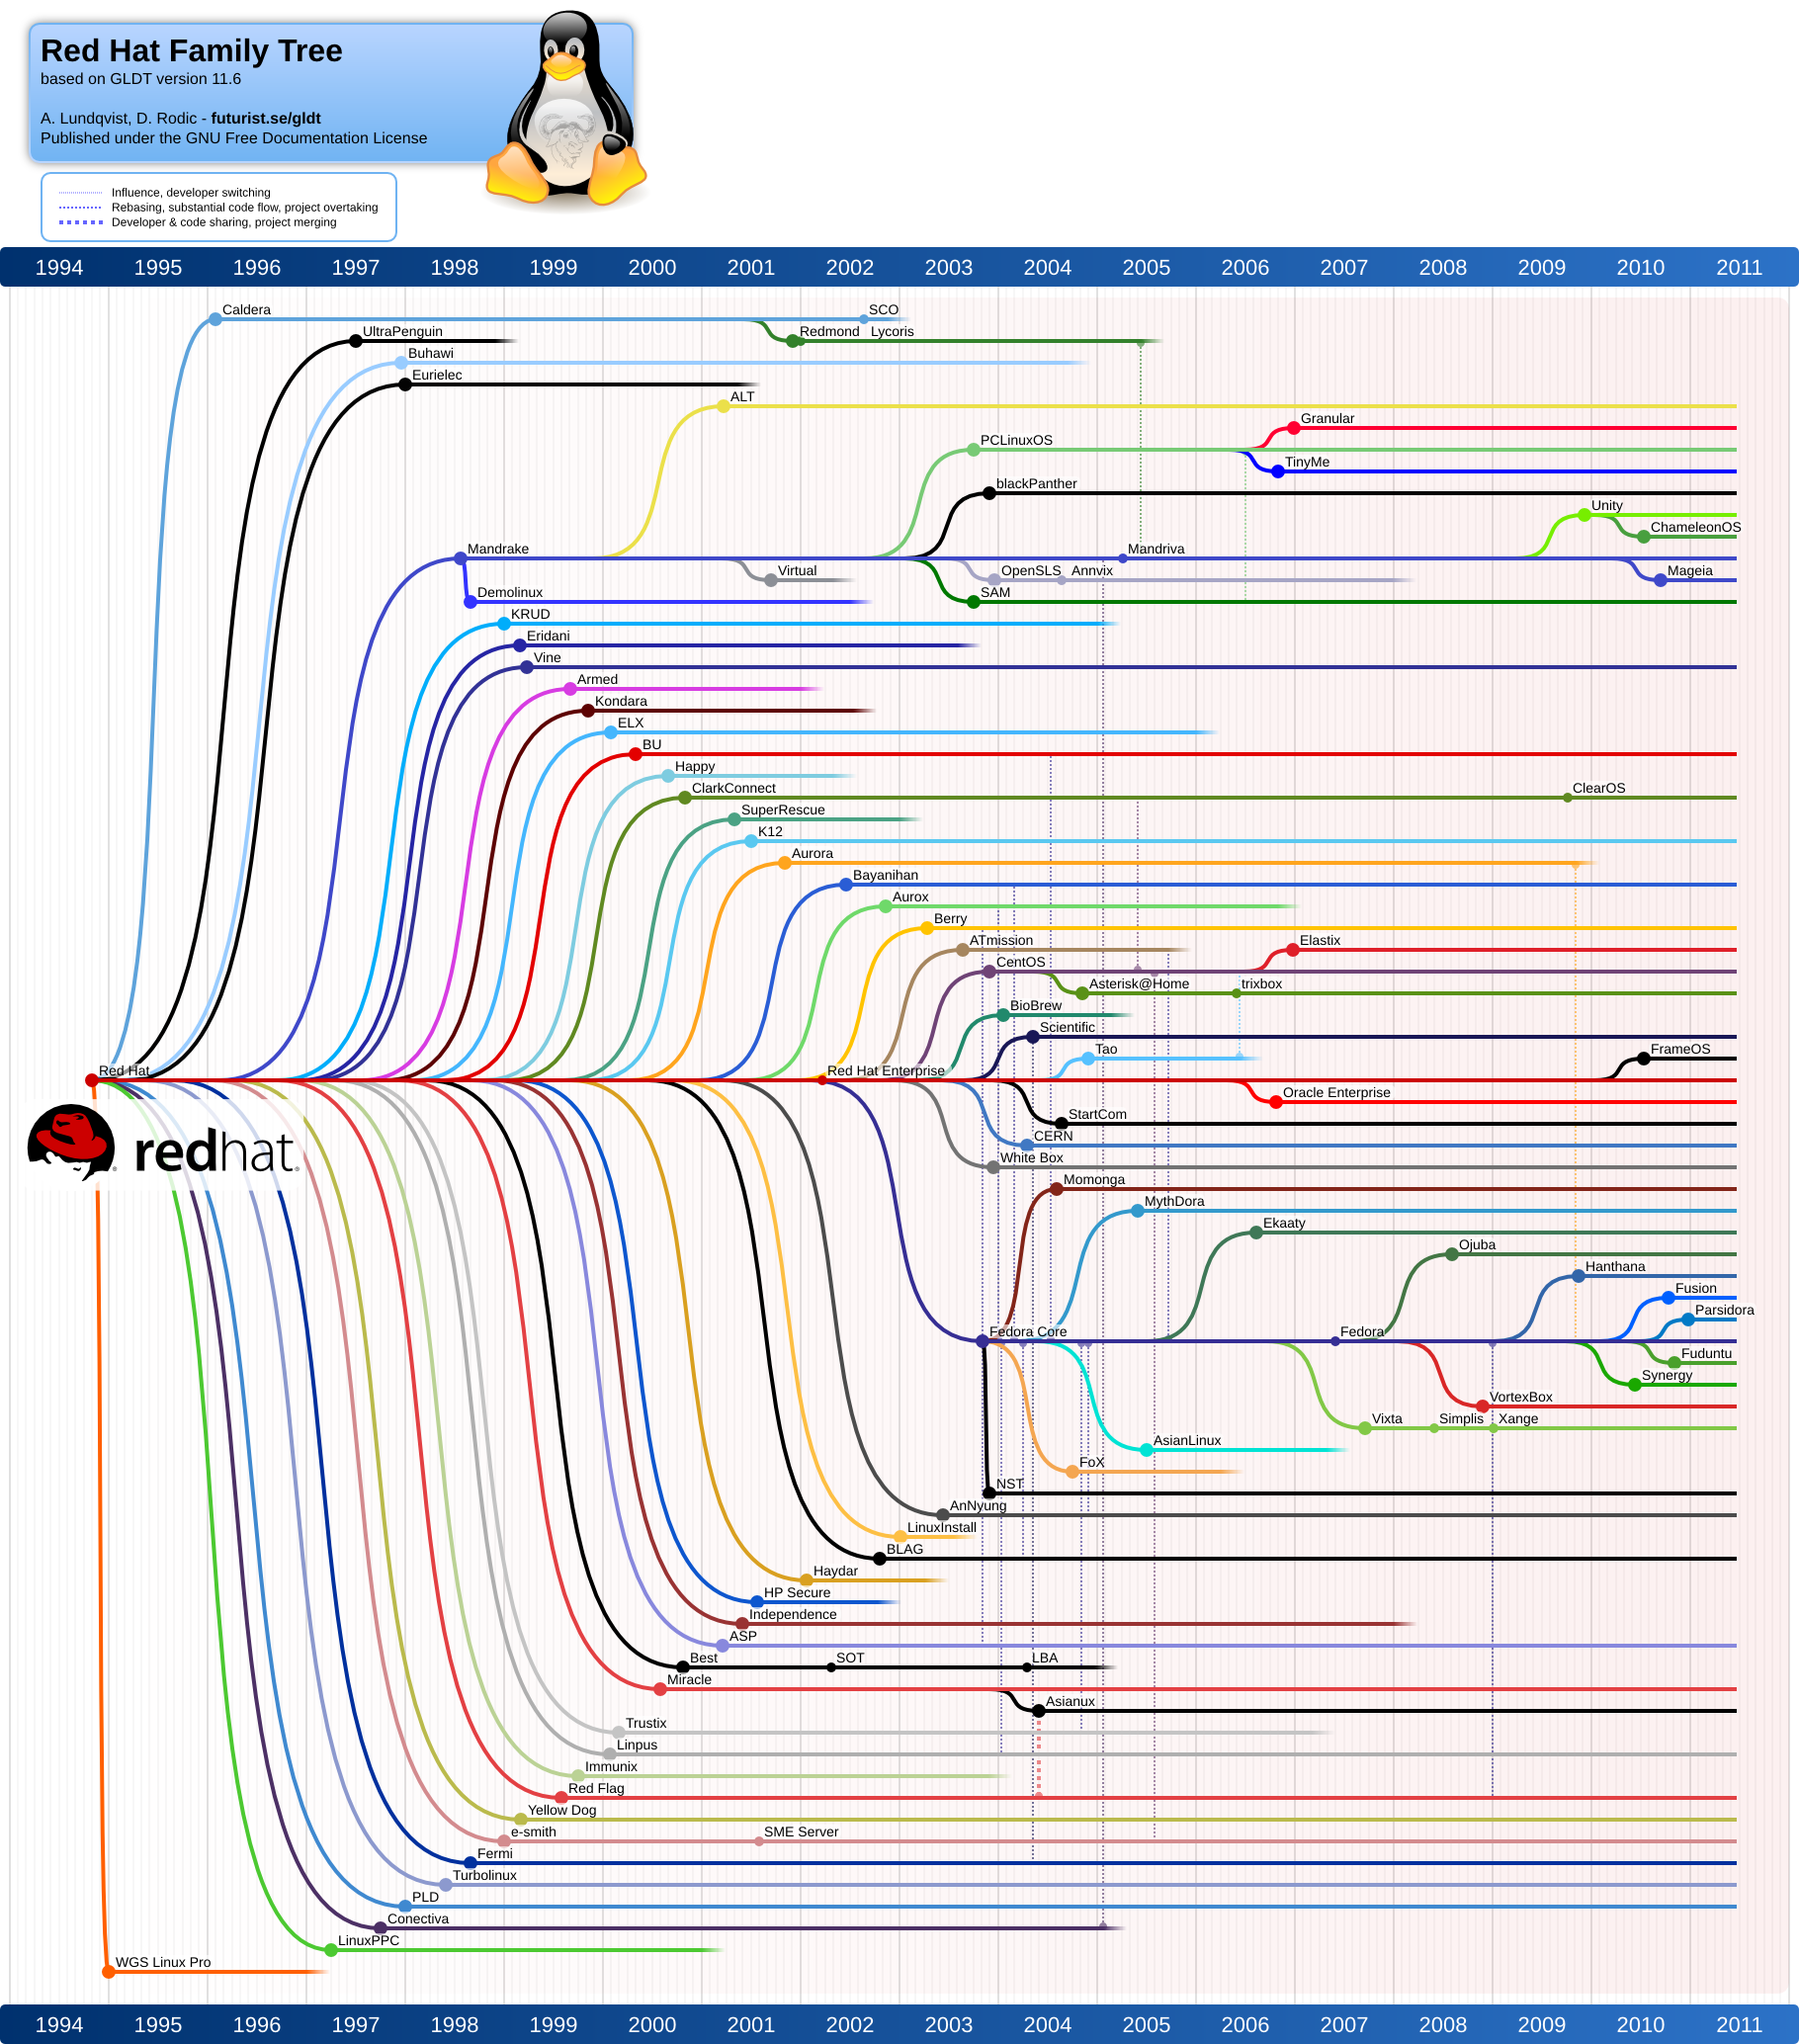
\includegraphics[width=0.85\textwidth]{figuras/redhat-timeline}
  \caption[Timeline RedHat]{Timeline ate 2011 da distribuição RedHat\protect\footnotemark.}
  \label{fig:figuras_linux_timeline_redhat}
\end{figure}

\footnotetext{\label{note:figuras_linux_timeline_redhat}\textbf{Fonte:} \href{https://upload.wikimedia.org/wikipedia/commons/a/a3/Redhat_family_tree_11-06.png}{http://futurist.se/gldt/}}

As figuras \ref{fig:figuras_linux_timeline_redhat}  e \ref{fig:figuras_linux_timeline_debian} apresentam as ramificações que surgiram cronologicamente nas distribuições Debian e RedHat. A linha na horizontal indica a \textit{timeline} da distribuição. O desaparecimento da linha indica que a distribuição foi descontinuada. As linhas na vertical podem indicar uma ramificação (nova distribuição criada a partir de uma antiga) ou a fusão de distribuições. Linhas na horizontal contendo um circulo no meio do tracejado indicam que alguma distribuição alterou o seu  nome (como foi o caso do S.u.S.E para SuSE no ano de 1998). 


\begin{figure}[h]
  \centering
	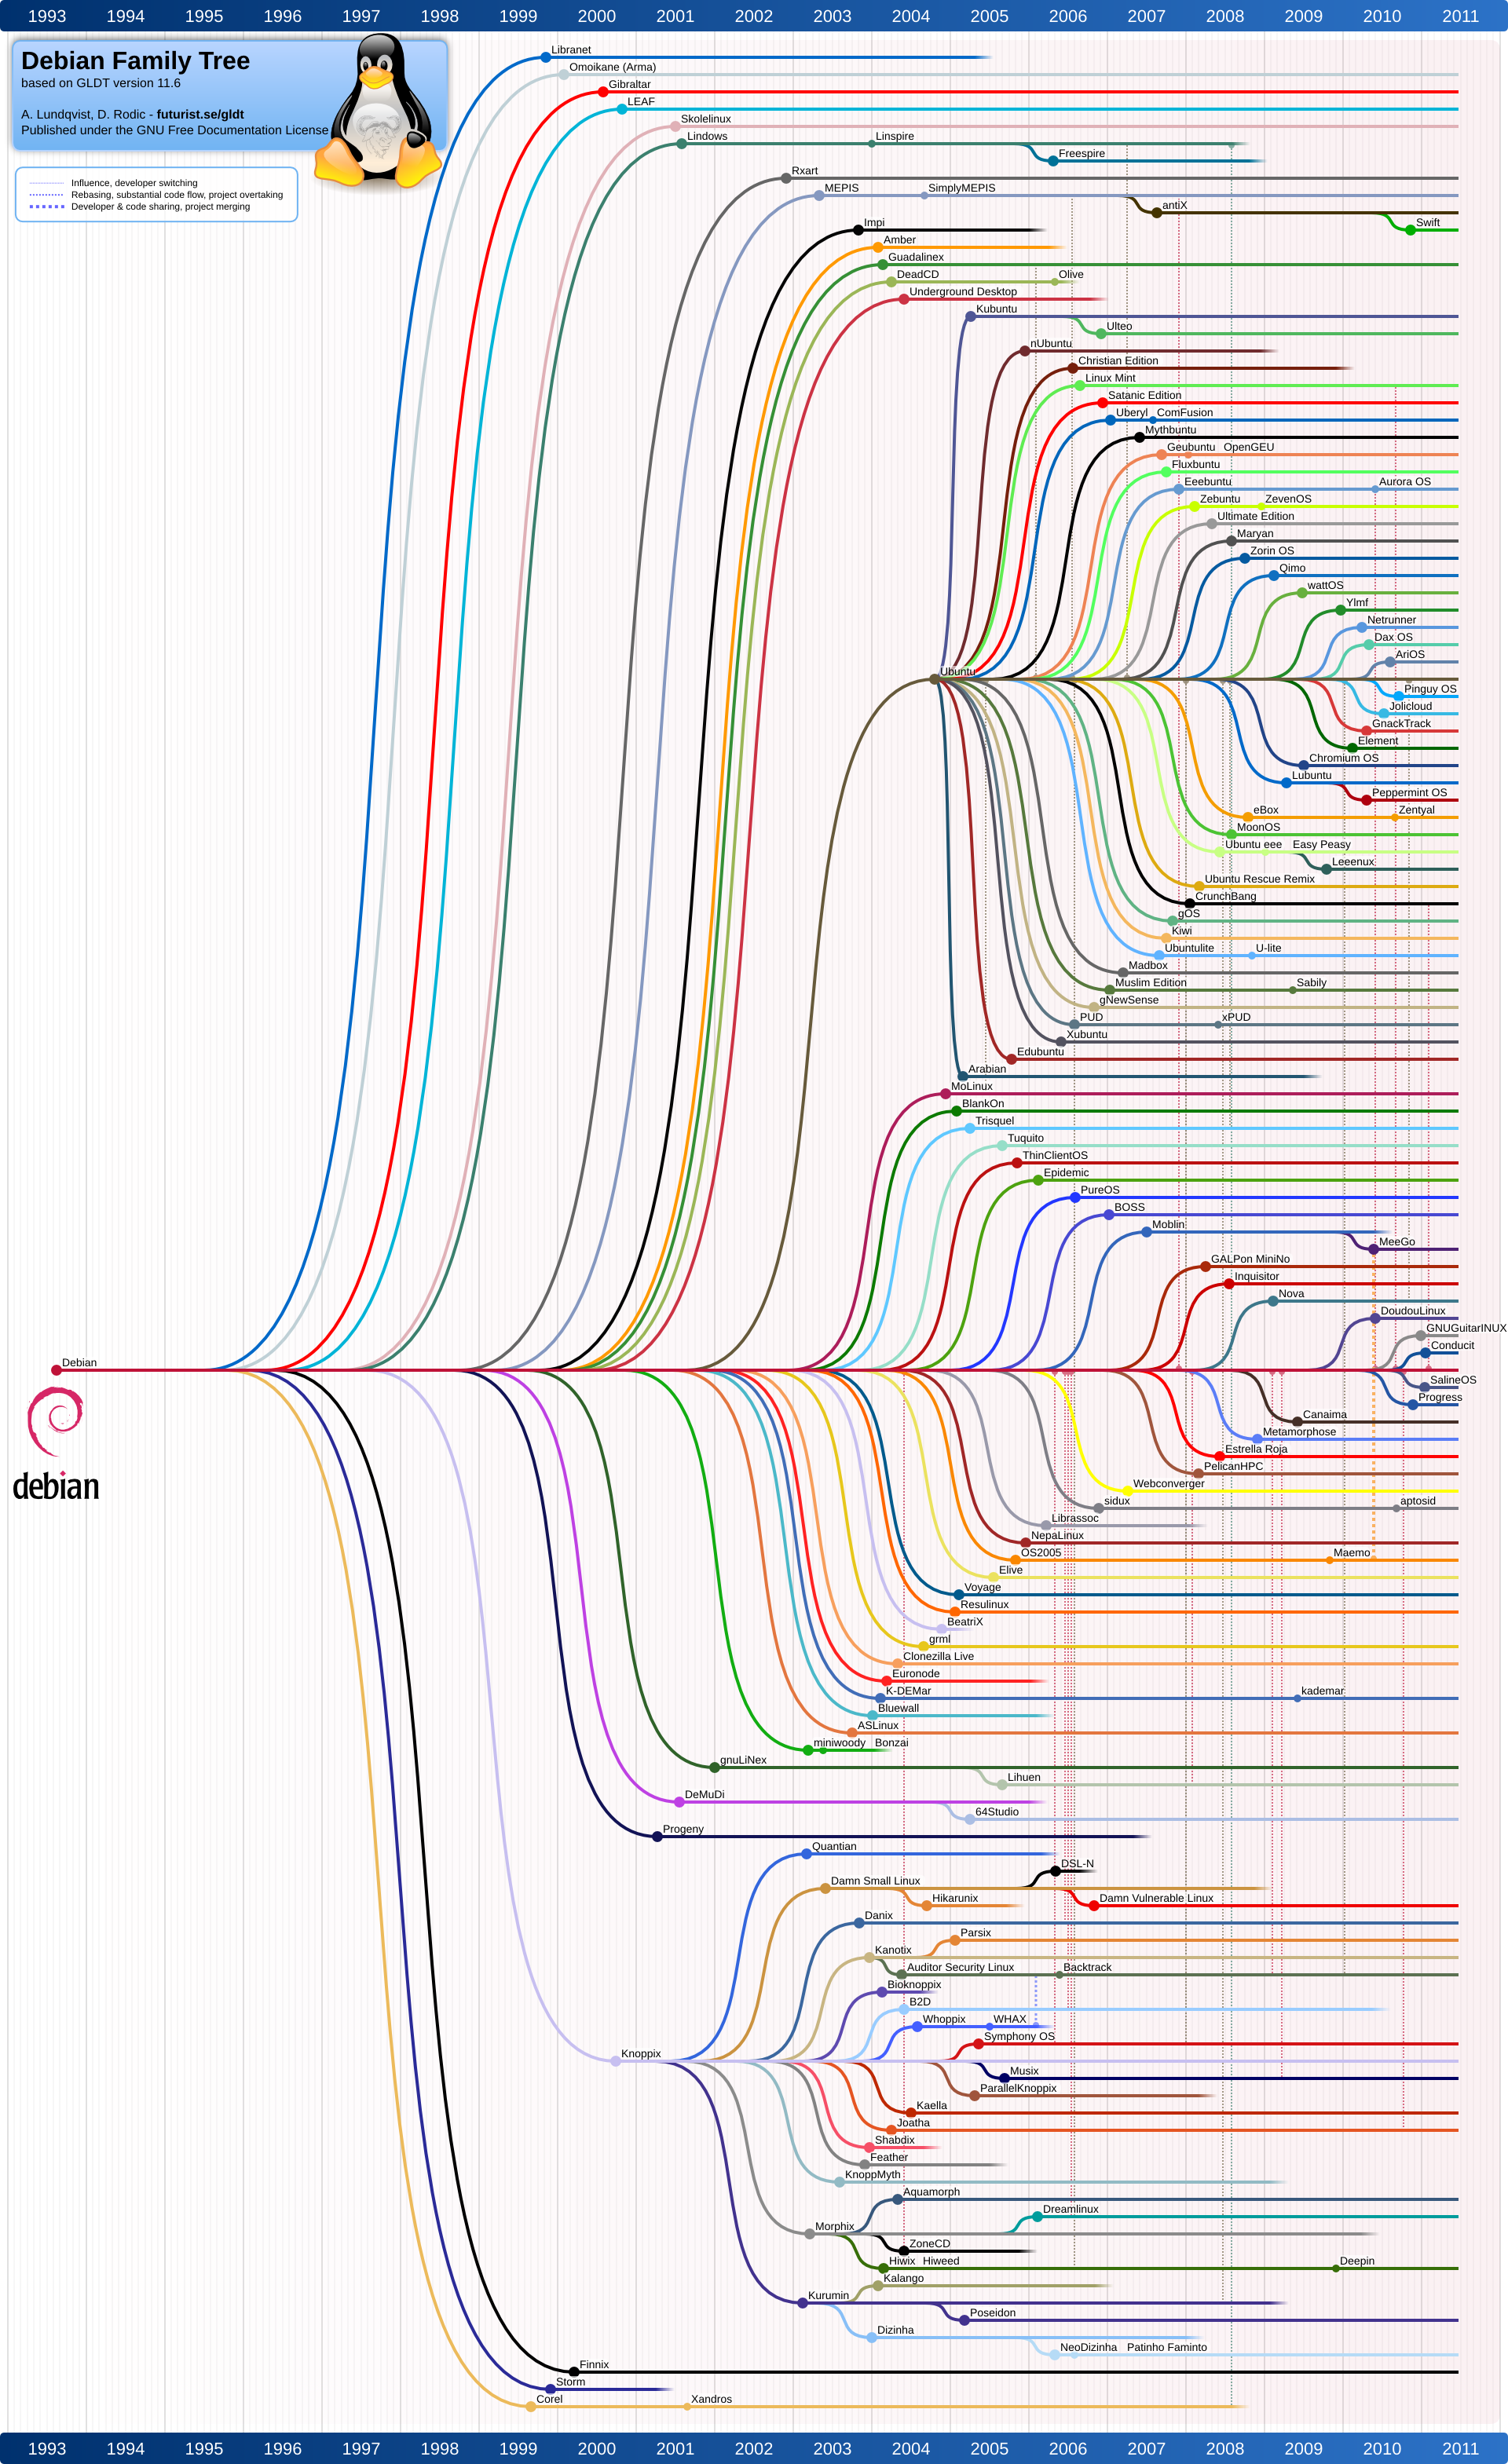
\includegraphics[width=0.7\textwidth]{figuras/debian-timeline}
  \caption[Timeline Debian]{Timeline ate 2011 da distribuição Debian\protect\footnotemark.}
  \label{fig:figuras_linux_timeline_debian}
\end{figure}

Mesmo que de dificil visualização do nome das distribuições na imagem, o objetivo dela no trabalho é contextualizar a influencia que as distribuições \textit{Debian} e \textit{Red Hat} tem entre diversas distribuições e que novas funcionalidades nelas serão eventualmente adotadas nas suas herdeiras, aumentando a propagação de funcionalidades. Assim, uma nova funcionalidade no \textit{Debian} certamente seria adotada na distribuição \textit{Ubuntu} e suas ramificações, porém novas funcionalidades no \textit{Ubuntu} demoram a serem copiadas para o \textit{Debian}, quando são. 
\footnotetext{\label{note:figuras_linux_timeline_debian}\textbf{Fonte:} \href{http://futurist.se/gldt/wp-content/uploads/subtrees/debian1106.png}{http://futurist.se/gldt/}}

As figuras são uma adaptação da imagem \textit{GNU/Linux Distribution Timeline}, a imagem pode ser melhor vizualizada em \url{http://futurist.se/gldt/wp-content/uploads/11.06/gldt1106.png}.

% Texto do segundo anexo.

\end{anexosenv}

